\lhead[\thepage]{CAPÍTULO \thechapter. EVALUACIÓN EXPERIMENTAL}
\chead[]{}
\rhead[Patrones de programación paralelos de alto nivel en arquitecturas de memoria distribuida\leftmark]{\thepage}
\renewcommand{\headrulewidth}{0.5pt}

\lfoot[]{}
\cfoot[]{}
\rfoot[]{}
\renewcommand{\footrulewidth}{0pt}

%% This is an example first chapter.  You should put chapter/appendix that you
%% write into a separate file, and add a line \include{yourfilename} to
%% main.tex, where `yourfilename.tex' is the name of the chapter/appendix file.
%% You can process specific files by typing their names in at the 
%% \files=
%% prompt when you run the file main.tex through LaTeX.
\chapter{Evaluación experimental}
\label{ch:evaluacion_experimental}
\markboth{}{EVALUACIÓN EXPERIMENTAL}

Este capítulo presenta la evaluación experimental de \acrshort{grppi} para plataformas de memoria distribuida. En primer lugar se describen los experimentos y la plataforma sobre la cual se han realizado (Sección \ref{sec:descripcion_experimentos}). Posteriormente se realiza un estudio de usabilidad (Sección \ref{sec:estudio_usabilidad}). Por último se realiza un análisis de rendimiento de la nueva implementación.

\section{Descripción de los experimentos}
\label{sec:descripcion_experimentos}

En esta sección, llevamos a cabo una evaluación experimental del back-end \acrshort{grppi} \acrshort{mpi} desde los puntos de vista de la usabilidad y el rendimiento. Para esta evaluación, empleamos los siguientes componentes de hardware y software:

\begin{itemize}

\item \textbf{Plataforma de destino}. La evaluación se ha llevado a cabo en un clúster homogéneo de ocho nodos, cada uno compuesto por un procesador Intel Xeon Broadwell E5-2603 v4 con 12 cores a 1.70\,GHz, 15\,MB de caché L3 y 128\,GB de \acrshort{ram} DDR3. El sistema operativo es Linux Ubuntu 16.04.3 LTS con el kernel 4.4.0-97. Los nodos están interconectados mediante un switch Ethernet de un Gigabit.

\item \textbf{Software}. Aprovechamos el nuevo back-end \acrshort{grppi} \acrshort{mpi} construido sobre \acrshort{grppi} v0.4~\cite{grppi-github}, junto con los respectivos back-end de memoria compartida y memoria distribuida, hilos de C ++11 y \acrshort{mpi}-3.1, implementados por \acrshort{mpi}CH v3.2.1. Tenga en cuenta que el back-end de \acrshort{mpi} se implementó con Boost \acrshort{mpi} v1.66.0. El compilador de C ++ utilizado para ensamblar \acrshort{grppi} fue GCC v7.2.0 que ya admite el estándar C ++ 14.

\item \textbf{Caso de uso}. Para evaluar los patrones distribuidos de Pipeline y Farm, aprovechamos una aplicación de transmisión que se encarga del cómputo de Mandelbrot, de forma que se crean imágenes para montar una animación de zoom fractal y aplicar el filtro de desenfoque gaussiano (Blur filter) en cada uno de los fotogramas generados. Concretamente, esta aplicación basada en Pipeline consta de las siguientes etapas:

\begin{description}
\item[Generador] devuelve valores de zoom crecientes monótonamente lineales, que se pasan a la etapa de Mandelbrot.
\item[Mandelbrot] toma el zoom recibido por el generador y calcula la trama de Mandelbrot correspondiente a dicho valor de zoom y las coordenadas del punto de interés.
\item[Gaussian blur] toma el frame calculado por la etapa anterior y aplica el filtro de desenfoque gaussiano a ellos, usando un kernel de 3$\times$3 píxels.
\item[Consumidor] guarda cada uno de los frames en el disco usando el formato BMP.
\end{description}

\end{itemize}

\vspace{0.35cm}
\begin{lstlisting}[linewidth=1\columnwidth,caption={Implementación Mandelbrot en Boost \acrshort{mpi}.},label=lst:mpimandelcode,frame=single]
int frame= 0;
int num_frames= 1000;
// Main Pipeline
grppi::Pipeline(mpi_exec,
  // Zoom generation
  [&]() -> std::experimental::optional<double> {
    if (frame++ == num_frames) return {};
      zoom-= zoom * 0.1;
    return zoom;
  },
  // Farm mandelbrot stage
  grppi::Farm(4,
    [&](auto zoom){
       return mandelbrot(height, width, poi_x, poi_y, zoom);
    }
  ),
  // Farm blur stage
  grppi::Farm(4,
    [&](auto image){
      return blur(height, width, kernel, image);
    }
  ), 
  // Consuming stage
  [&](auto image){
    save_bmp(height, width, image);
  }
);
\end{lstlisting}
\vspace{0.35cm}

Como se sabe generalmente, el conjunto de Mandelbrot es el conjunto de números complejos $c$ para los cuales la función $f_{c}(z)=z^{2}+c$ no diverge cuando se itera desde $z=0$, es decir, para el cual la secuencia $f_{c}(0)$, $f_{c}(f_{c}(0))$, etc., permanece limitada en valor absoluto. Por lo tanto, las imágenes de Mandelbrot pueden crearse muestreando los números complejos y determinando, para cada punto de muestra $c$, si el resultado de iterar la función anterior va al infinito. Luego, tratando las partes real e imaginaria de $c$ como coordenadas de imagen $(x+yi)$ en el plano complejo, los píxeles pueden colorearse de acuerdo con la rapidez con la secuencia $z_{n}^{2}+c$ diverge. Esta es la clave para comprender la naturaleza heterogénea de esta operación, donde la velocidad de divergencia en el punto de interés y el valor del zoom dictan el número de iteraciones para calcular un frame dado. Por el contrario, el operador de desenfoque gaussiano tiene una carga de trabajo casi homogénea para procesar cada uno de los frames. En nuestro caso de uso específico, el caso de uso de Mandelbrot se configuró para generar 1,000 frames y hasta 1,000 iteraciones para calcular cada frame del Mandelbrot.

\vspace{0.35cm}
\begin{lstlisting}[linewidth=1\columnwidth,caption={Implementación Mandelbrot en \acrshort{grppi} \acrshort{mpi}.},label=lst:grppimandelcode,frame=single]
std::vector<color> image;
if (world.rank() == 0) { // Zoom generator
  for(int frame= 0; frame < num_frames; frame++) {
    zoom-= zoom * 0.1;
    world.send(world.rank()+1, 0, zoom);
  }
}
else if (world.rank() == 1) { // Mandelbrot stage
  for(int frame= 0; frame < num_frames; frame++) {
    world.recv(world.rank()-1, 0, zoom);
    image = mandelbrot(height, width, poi_x, poi_y, zoom);
    world.send(world.rank()+1, 0, image);
  }
}
else if (world.rank() == 2) { // Blur stage
  for(int frame= 0; frame < num_frames; frame++) {
    world.recv(world.rank()-1, 0, image);
    image = blur(height, width, kernel, image);
    world.send(world.rank()+1, 0, image);
  }
} 
else if (world.rank() == 3) { // Consuming stage
  for(int frame= 0; frame < num_frames; frame++) {
    world.recv(world.rank()-1, 0, image);
    save_bmp(height, width, image);
  }
}
\end{lstlisting}
\vspace{0.35cm}

Dado el paralelismo natural de esta aplicación, donde cada uno de los fotogramas de animación se puede calcular de forma independiente, las etapas del Pipeline Mandelbrot y Gaussian blur pueden ser replicadas mediante el patrón Farm, por lo que pueden procesar fotogramas individuales. Por lo tanto, pueden surgir varias composiciones dependiendo de la paralelización de estas etapas, es decir, \texttt{(p|p|p|p)}, \texttt{(p|f|p|p)}, \texttt{(p|p|f|p)}, y \texttt{(p|f|f|p)}.

% As studied in Exercise~\ref{mandelbrot}, images of the Mandelbrot set exhibit an elaborate and infinitely complicated boundary that reveals progressively ever-finer recursive detail at increasing magnifications of the core function (remember the \texttt{zoom} variable). The ``style'' of this repeating detail depends on the region of the set being examined. The set's boundary also incorporates smaller versions of the main shape, so the fractal property of self-similarity applies to the entire set, and not just to its parts.

En las secciones siguientes, analizamos la usabilidad y el rendimiento de los patrones \acrshort{grppi} Pipeline y Farm distribuidos utilizando el punto de referencia mencionado anteriormente con diferentes configuraciones de grado de paralelismo con respecto al número de procesos \acrshort{mpi} y subprocesos de trabajo utilizados en las etapas de Farm. Además, evaluamos los costes del uso de \acrshort{grppi} con respecto a la paralelización directa de la aplicación a través de \acrshort{mpi}.

\section{Estudio de la usabilidad}
\label{sec:estudio_usabilidad}

Para analizar la usabilidad y la productividad de la interfaz de patrones propuesta y el nuevo back-end de \acrshort{mpi}, utilizamos la herramienta analizadora Lizard~\cite{lizard} para obtener dos métricas bien conocidas: Líneas de código (LOCs) y el Número de Complejidad Ciclomática de McCabe's (CCN)~\cite{McCabe:1976}. Básicamente, utilizamos estas métricas para analizar las diferentes versiones de casos de uso, es decir, con y sin utilizar la interfaz \acrshort{grppi}. La Tabla~\ref{tab:lines} resume el porcentaje de LOCs adicionales introducidos en el código fuente secuencial para implementar las versiones paralelas usando \acrshort{mpi} y la interfaz \acrshort{grppi}, junto con sus CCNs correspondientes. Como se observa, la implementación de composiciones más complejas a través de \acrshort{mpi} conduce a códigos fuente más grandes y más complejos, mientras que para \acrshort{grppi} el número de LOCs radicionales permanece constante. Esta diferencia se debe principalmente a las colas de comunicación requeridas para implementar el patrón Farm. Centrándonos en \acrshort{grppi}, observamos que el esfuerzo de paralelización es casi insignificante: incluso la composición más compleja aumenta casi el 4.2\,\% de LOCs. Además, al cambiar a \acrshort{grppi} para que use una política de ejecución particular, solo se necesita cambiar un único argumento en la llamada a la función de patrón. Con respecto a la complejidad ciclomática para \acrshort{mpi}, observamos que sus CCNs son aproximadamente proporcionales al aumento del porcentaje de LOCs. . Por el contrario, la interfaz \acrshort{grppi} tiene CCN constantes para todas las composiciones de Pipeline.

\vspace{0.35cm}
\newcolumntype{C}{>{\centering\let\newline\\\arraybackslash\hspace{0pt}}p{1.2cm}}
\begin{table}[ht!]
\centering
%\vspace{-0.8cm}
\caption{Porcentaje de LOCs adicionales con respecto a la versión secuencial y los CNNs para las composiciones de Pipeline.}\label{tab:lines}\vspace{-0.15cm}
\small
\scalebox{1}{
\begin{tabular}{|c|C|C|C|C|}\hline
%  Pipeline  & \multicolumn{2}{c|}{\textbf{MPI}}  & \multicolumn{2}{c|}{\textbf{\acrshort{grppi}}}\\\cline{2-5}
% composición & LOCs & CCNs & LOCs & CCNs \\\hline\hline
% \texttt{(p|p|p|p)}  & $+$75.1\,\%  & 18  & $+$4.2\,\%   & 7  \\
% \texttt{(p|f|p|p)}  & $+$130.4\,\% & 38  & $+$4.2\,\%   & 7  \\
% \texttt{(p|p|f|p)}  & $+$130.4\,\% & 38  & $+$4.2\,\%   & 7  \\
% \texttt{(p|f|f|p)}  & $+$185.8\,\% & 58  & $+$4.2\,\%   & 7  \\\hline

 Composición  & \multicolumn{2}{c|}{\textbf{\% LOCs adicionales}}  & \multicolumn{2}{c|}{\textbf{CCN}} \\\cline{2-5}
Pipeline & \acrshort{mpi} & \acrshort{grppi} & \acrshort{mpi} & \acrshort{grppi} \\\hline\hline
\texttt{(p|p|p|p)}  & $+$10.3\,\%  & $+$4.2\,\% & 9 & 7  \\
\texttt{(p|f|p|p)}  & $+$130.4\,\% & $+$4.2\,\% & 38 & 7  \\
\texttt{(p|p|f|p)}  & $+$130.4\,\% & $+$4.2\,\% & 38 & 7  \\
\texttt{(p|f|f|p)}  & $+$185.8\,\% & $+$4.2\,\% & 58 & 7  \\\hline
\end{tabular}}
%\vspace{-0.7cm}
\end{table}
\vspace{0.35cm}

Finalmente, realizamos una comparación lado a lado entre las interfaces Boost \acrshort{mpi} y \acrshort{grppi} implementando una versión simplificada del caso de uso de Mandelbrot. % As can be seen in Listing~\ref{lst:grppimandelcode}, the \grppi code follows a comprehensible and readable structure, which clearly shows the compositions among stream operators. On the contrary, the \acrshort{mpi} code, shown in Listing~\ref{lst:mpimandelcode}, is not as structured and easy to read as the \grppi implementation.\footnote{For the sake of simplicity, we have replaced the use of queues by synchronous communications, so no computations overlap communications in this case.} 
Como se puede ver en el Listado \ref{lst:mpimandelcode}, la implementación de \acrshort{mpi} distingue claramente las instrucciones y comunicaciones que deben ser ejecutadas por cada uno de los procesos. \footnote{Para mayor simplicidad, hemos reemplazado el uso de colas por comunicaciones síncronas, por lo que no hay cálculos que se superpongan a las comunicaciones en este caso.}. Por otro lado, el código \acrshort{grppi}, que se muestra en el Listado~\ref{lst:grppimandelcode}, se centra más en la estructura del algoritmo de la aplicación que en las comunicaciones entre procesos.
%follows a comprehensible and readable structure, which clearly shows the application algorithm structure. 
%is more structured and easier to read than the \acrshort{mpi} implementation.
%Thus, to properly understand the application behavior, users need to carefully analyze its structure along with the execution flow to known which portions of the code will be executed by each of the processes.
En pocas palabras, aunque ambas interfaces proporcionan interfaces de alto nivel, concluimos que las implementaciones de patrones ofrecidas por \acrshort{grppi} ayudan a mejorar tanto la productividad como la capacidad de mantenimiento.

\section{Análisis de rendimiento}
\label{sec:analisis_rendimiento}

En esta sección, evaluamos el rendimiento y la escalabilidad de la aplicación Mandelbrot implementada con la interfaz \acrshort{grppi} utilizando la política \acrshort{mpi} junto con el back-end de memoria compartida basado en hilos C ++ 11. Evaluamos el rendimiento de la aplicación utilizando solo el back-end de memoria compartida. Además, hemos limitado la cantidad de núcleos por nodo para simular diferentes escenarios de clúster. Tenga en cuenta que solo nos centramos en la composición del Pipeline \texttt{(p|f|f|p)}, ya que ofrece el mejor rendimiento y puede escalarse mejor entre los nodos del clúster.

La Figura~\ref{fig:mandel-pffp} representa la escala de speedup cuando se usa de 1 a 8 nodos de clúster y se ejecuta de 1 a 12 subprocesos por nodo para resoluciones de cuadros cuadrados de 200, 400 y 800 píxeles con respecto a la aplicación secuencial. Es importante destacar que cada experimento ejecuta tantos operadores (etapas de Pipeline y réplicas de Farm) como la cantidad total de subprocesos ejecutados en los nodos. Como se observa, el speedup logrado por \acrshort{mpi} usando un solo nodo es igual a la memoria compartida; esto viene dado por el hecho de que el back-end \acrshort{mpi} delega completamente en el back-end de la memoria compartida cuando se ejecuta en un nodo. En este primer intento del experimento, establecemos el mismo número de réplicas de Farm en las etapas de Mandelbrot y de Gaussian Blur. Como puede verse, para 1, 2 y 4 nodos, la aplicación escala linealmente con el número de subprocesos por nodo, con una eficiencia sostenida de aproximadamente 45\,\%. Sin embargo, para 8 nodos, el rendimiento se degrada desde 6 subprocesos por nodo, ya que la etapa de Mandelbrot causa un importante cuello de botella en la interconexión debido a los niveles de producción desequilibrados. La eficiencia máxima, en este caso, es 26\,\%. Esto se debe a que la carga de trabajo de Mandelbrot por cada frame es mucho mayor que la aplicación del operador Gaussian Blur.

Para lidiar con este desequilibrio, hemos calculado empíricamente la relación entre los rendimientos de las etapas Mandelbrot y Blur, que nos sirvió para determinar el número óptimo de réplicas en las etapas correspondientes de Farm. Básicamente, hemos calculado esta relación usando promedios de rendimiento de ambas etapas para las diferentes resoluciones de frame. Usando esta proporción, asignamos 1 réplica de Blur por cada 25 réplicas de Mandelbrot. Sin embargo, esta relación no ofrece rendimientos ideales dada la naturaleza heterogénea de la carga de trabajo del conjunto de Mandelbrot. La Figura~\ref{fig:mandel-pfsp} muestra el rendimiento logrado para la diferente cantidad de nodos y subprocesos por experimentos de nodo y el uso de la relación antes mencionada. Como se observa, de 1 a 4 nodos, la eficiencia mejora significativamente con respecto al experimento anterior, de 45\,\% a 68\,\%. Los resultados también revelan escalas de rendimiento relativamente buenas para todos los tamaños de frame.  Por otro lado, para 8 nodos, la aplicación muestra un peor rendimiento cuando se utilizan más de 6 subprocesos por núcleo. Esta degradación se debe principalmente a la diferencia entre la carga de trabajo de la etapa y los gastos generales de comunicación inherentes. Por esta razón, para tamaños de cuadros grandes, el rendimiento alcanzado es ligeramente mejor, ya que los cálculos paralelos pagan los tiempos de serialización y transferencia de datos requeridos. En cualquier caso, para 8 nodos, la eficiencia obtenida usando etapas de Farm equilibradas aumenta de 26\,\% a 45\,\%.

\vspace{0.35cm}
\begin{figure}[!tbp]
\centering
\begin{subfigure}[b]{0.32\textwidth}
  \centering
  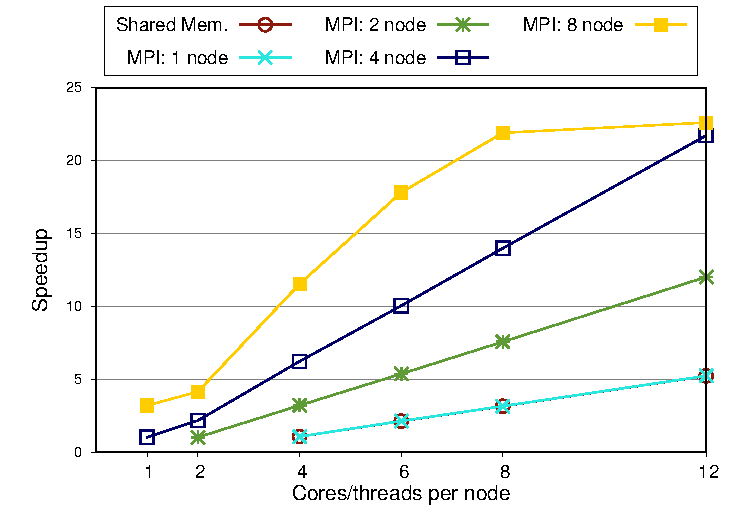
\includegraphics[width=0.95\linewidth]{figures/graph-mpi-200-pffp.pdf}
  \caption{Resolución de imagen 200$\times$200.}
  \label{fig:mandel-pffp-200}
\end{subfigure}%
\hfill
\begin{subfigure}[b]{0.32\textwidth}
  \centering
  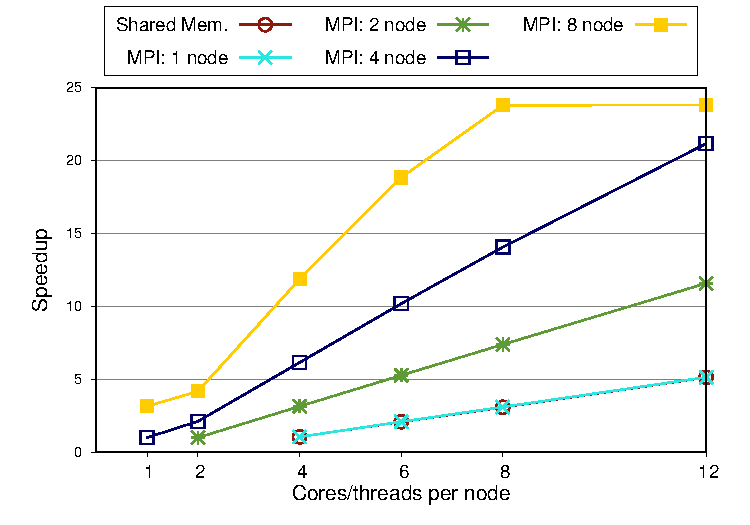
\includegraphics[width=0.95\linewidth]{figures/graph-mpi-400-pffp.pdf}
  \caption{Resolución de imagen 400$\times$400.}
  \label{fig:mandel-pffp-400}
\end{subfigure}
\hfill
\begin{subfigure}[b]{0.32\textwidth}
  \centering
  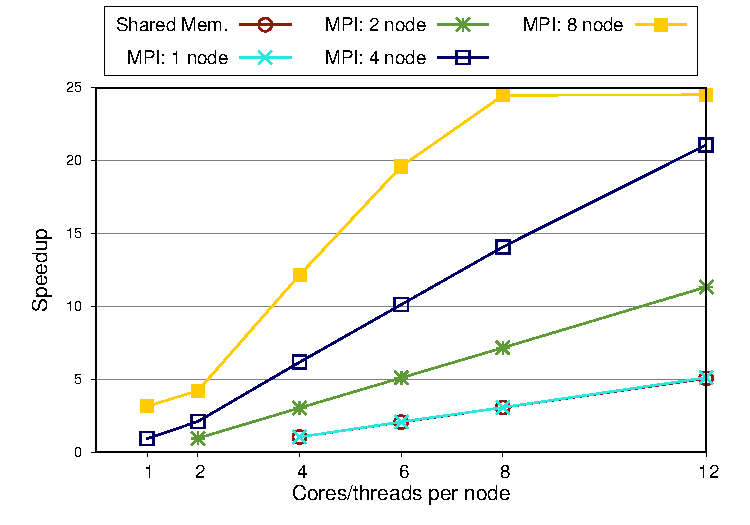
\includegraphics[width=0.95\linewidth]{figures/graph-mpi-800-pffp.pdf}
  \caption{Resolución de imagen 800$\times$800.}
  \label{fig:mandel-pffp-800}
\end{subfigure}
\caption{Caso de uso de Mandelbrot con Pipeline \texttt{(p|f|f|p)} con mismo número de réplicas de Farm.}
\label{fig:mandel-pffp}
\end{figure}
\vspace{0.35cm}

A partir de estos experimentos, podemos concluir que la interfaz \acrshort{grppi} propuesta puede ayudar a implementar aplicaciones científicas de flujo distribuido a expensas de gastos indirectos insignificantes. En un experimento separado, evaluamos la sobrecarga introducida por \acrshort{grppi} con respecto a utilizar \acrshort{mpi} directamente. Esta sobrecarga fue menor a 0.1\,\%.

\vspace{0.35cm}
\begin{figure}[!tbp]
\centering
\begin{subfigure}[b]{0.32\textwidth}
  \centering
  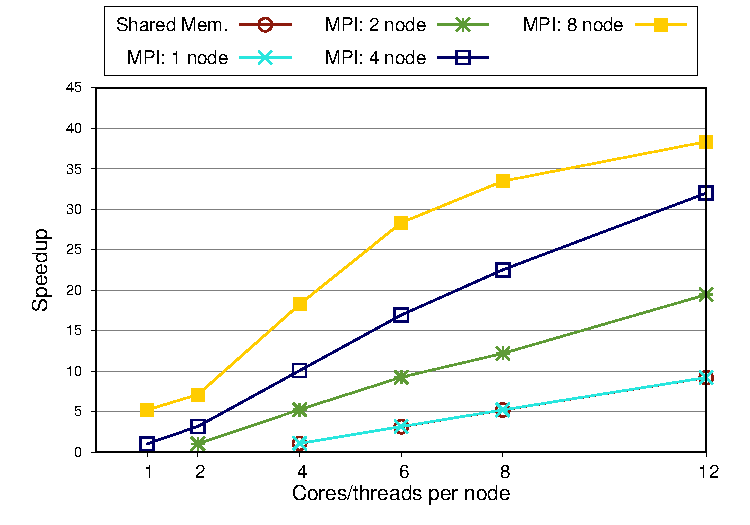
\includegraphics[width=0.95\linewidth]{figures/graph-mpi-200-pfsp.pdf}
  \caption{Resolución de imagen 200$\times$200.}
  \label{fig:mandel-pfsp-200}
\end{subfigure}%
\hfill
\begin{subfigure}[b]{0.32\textwidth}
  \centering
  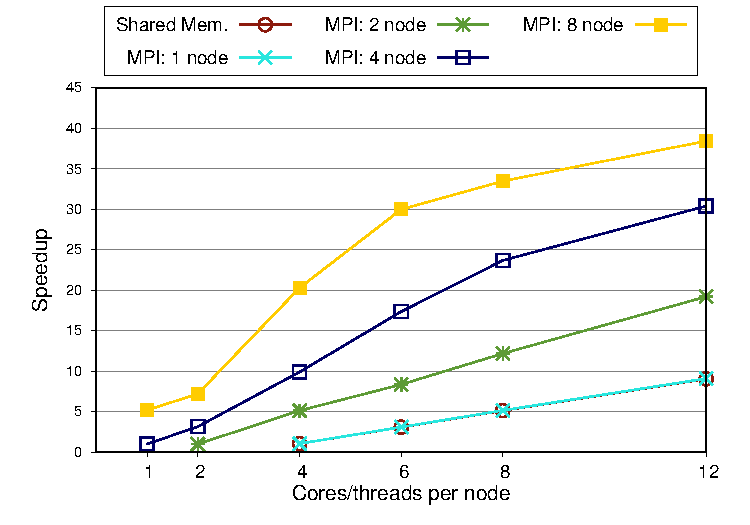
\includegraphics[width=0.95\linewidth]{figures/graph-mpi-400-pfsp.pdf}
  \caption{Resolución de imagen 400$\times$400.}
  \label{fig:mandel-pfsp-400}
\end{subfigure}
\hfill
\begin{subfigure}[b]{0.32\textwidth}
  \centering
  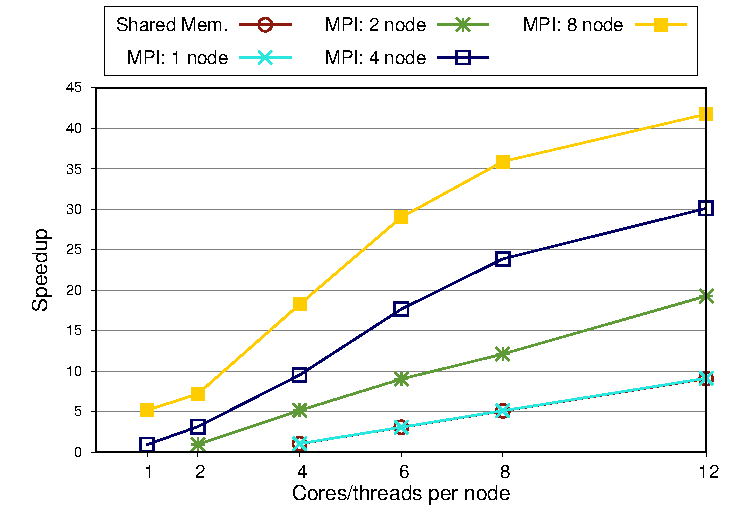
\includegraphics[width=0.95\linewidth]{figures/graph-mpi-800-pfsp.pdf}
  \caption{Resolución de imagen 800$\times$800.}
  \label{fig:mandel-pfsp-800}
\end{subfigure}
\caption{Caso de uso de Mandelbrot con Pipeline \texttt{(p|f|f|p)} con un número ajustado de réplicas de Farm.}
\label{fig:mandel-pfsp}
\end{figure}
\vspace{0.35cm}

%\afterpage{\blankpage} % blank page